\begin{abstract}
在机会只能获得一次奖励、增加搜索资源会提高捕获概率的环境中，少量收入试验能支持怎样的投入决策？本文把投入强度建模为连续变量，不预设未知机会的数量和组成。给定三个等距测试点的平均收入，利用矩约束求出不能进一步缩小的收入范围，并据此计算最高可能利润和最优保守投入。两者都来自同一组模型约束，但对测量误差的要求不同：当单位资源费用低于一个由读数决定的阈值时，准确报告最高可能利润需要随最大部署强度平方增长的观测次数；保守投入的充分观测次数则可以不随该上限增长。已知总奖励上限会使这种增长最终停止。一个已知有限机会数、只有单位奖励的构造说明，即使允许连续选择低强度试验，饱和前的统计困难仍然存在。数值部分只保留一个有限机会池案例，展示利润范围、连续投入选择和含噪数据下的完整停止过程。全部结果由本机重新执行程序生成；案例为合成数据，尚不构成真实市场的应用验证。
\end{abstract}
\noindent\textbf{关键词：}资源配置；部分识别；稳健优化；测量精度；机会捕获

\section{研究问题}
一个团队可以增加搜索吞吐或处理能力，却不能直接观察全部潜在机会。它只知道若干资源水平下的平均收入，需要判断进一步扩张是否值得，以及当前信息支持多大的投入。本文研究这类有限信息下的资源配置问题。

少量试验通常不能确定完整的收入曲线。直接拟合一条曲线再求最优投入，会把无法识别的部分当成已知。本文保留所有与试验结果一致的收入模型，先计算它们允许的利润范围，再讨论这一范围能支持什么决策。范围的上端可用于排除收益不足的扩张目标；范围的下端对应一个不依赖具体模型的保守投入。上端不是收益预测，下端也不是每次经营都能实现的现金回报。

本文集中说明两个结果。第一，三个等距测试点已经足以显式计算整个连续投入区间上的最紧收入上下界。第二，扩大可部署规模时，排除高利润可能性所需的精度，可能比选取保守投入所需的精度严格得多。后一个结果有明确的费用条件与奖励上限条件，不适用于所有市场。

计算工具来自经典矩问题\cite{dette}、极小极大定理\cite{sion}和统计检验下界。利用置信集合支持决策也已有成熟研究\cite{bgk}；预测精度与决策损失的差别并非本文首次提出\cite{spo}。本文讨论的是这一具体机会机制下可计算的利润范围、费用阈值及测量需求，不把上述通用方法列为新贡献。

\section{连续投入、收入模型与试验信息}
\subsection{投入怎样产生收入}
固定一个经营窗口。投入强度 $q\geq0$ 表示相对搜索或处理能力，$q=1$ 为基准水平；它不是交易本金。对于第 $i$ 类机会，设一次成功获得奖励 $R_i\geq0$，基准累计有效命中强度为 $z_i>0$。若尝试服从泊松时钟，增加投入把时钟速率乘以 $q$，则窗口内至少命中一次的概率为 $1-e^{-qz_i}$。每个机会只结算一次奖励。因此
\begin{equation}\label{eq:model}
 P_\nu(q)=\int_{(0,\infty)}(1-e^{-qz})\,\nu(dz),
 \qquad f_\nu(q)=P_\nu(q)-cq.
\end{equation}
有限机会时，积分就是 $\sum_i R_i(1-e^{-qz_i})$。测度 $\nu$ 按捕获速度汇总奖励，不是概率分布；其总质量是总奖励。$P_\nu$ 是每窗口期望收入，$c>0$ 是每单位强度的资源费用，$f_\nu$ 是期望净利润。允许的部署区间为 $[0,Q]$，不执行的利润为零。

式\eqref{eq:model}隐含两项实质假设：资源线性提高有效尝试率；奖励和机会组成不因本次投入而变化。它给出的收入递增且凹，但比一般的递增凹函数更受限制。该指数核也见于泊松占据模型\cite{gnedin}。如果投入同时改变竞价、滑点、目标人群或竞争者行为，不能直接沿用此响应。

\subsection{为什么测试三个点，而投入仍然连续}
一般可在任意连续强度 $t_1,\ldots,t_m>0$ 上试验。记准确均值为 $p_i=P_\nu(t_i)$，所有与这些均值一致的模型为
\begin{equation}\label{eq:modelset}
 \calM(p;t)=\left\{\nu\geq0:\nu((0,\infty))<\infty,
 \ \int(1-e^{-t_i z})\nu(dz)=p_i\ (i=1,\ldots,m)\right\}.
\end{equation}
这个定义没有把 $q$ 限制为整数。本文的显式公式选择 $t_1=h,t_2=2h,t_3=3h$。把资源单位改成 $h$ 后，测试点写成 $1,2,3$，相应单位费用改为 $ch$。选择等距点的理由是代数可解，而不是实际投入只有三个档位，更不是三个点已经被证明为最优试验设计。

具体地，令 $v=1-e^{-z}\in(0,1)$，则三个读数分别包含 $v$、$2v-v^2$ 和 $3v-3v^2+v^3$。因此它们等价于三个普通矩。任意不等距点仍可使用\eqref{eq:modelset}计算上下界，只是不能直接套用后面的闭式公式。第\ref{sec:numerics}节给出不等距测试点的数值对照。是否应当根据数据选择最优测试强度，本文没有解决。

在确定性分析中先把 $p$ 当作已知；统计分析再从重复观测中估计它。两个阶段不可混淆：三个平均收入不等于只做三次随机试验。

\section{三个读数支持怎样的利润判断}
\subsection{收入范围和最优保守投入}
以下用 $\calM(p)$ 表示测试点为 $1,2,3$ 的模型集合。对连续投入 $q>0$ 定义
\begin{equation}\label{eq:envelopes}
 L(p,q)=\inf_{\nu\in\calM(p)}P_\nu(q),\qquad
 U(p,q)=\sup_{\nu\in\calM(p)}P_\nu(q).
\end{equation}
真实模型的最优利润、最高可能利润和最优保守保证分别为
\begin{align}
 V(\nu)&=\max_{0\leq q\leq Q}\{P_\nu(q)-cq\},\notag\\
 \Vup(p,Q,c)&=\sup_{\nu\in\calM(p)}V(\nu),\label{eq:values}\\
 \Vlo(p,Q,c)&=\max_{0\leq q\leq Q}\{L(p,q)-cq\}.\notag
\end{align}
实现最后一项的投入记为 $\qrob$。它保证每个与试验一致的模型都有 $f_\nu(\qrob)\geq\Vlo$，但不保证接近该模型自己的 $V(\nu)$。因此，不能把后文的保守行动精度说成真实最优行动精度。

令
\begin{equation}\label{eq:moments}
 a=p_1,\qquad b=2p_1-p_2,\qquad d=3p_1-3p_2+p_3.
\end{equation}
记 $\mu$ 为按 $v=1-e^{-z}$ 重新归类后的奖励测度，则 $a,b,d$ 分别为 $\int v\,\mu(dv)$、$\int v^2\,\mu(dv)$ 和 $\int v^3\,\mu(dv)$。假设 $a>b>d>0$ 且 $ad>b^2$，即读数处于严格的矩可行域内部。设
\begin{align}
 r&=a-\frac{b^2}{d},&s&=\frac db,&A&=\frac{b^3}{d^2},\notag\\
 \ell&=\frac{b-d}{a-b},&w&=\frac{a-b}{1-\ell},&m_0&=a-w,\label{eq:parameters}\\
 F(p,q)&=rq+A[1-(1-s)^q],&&\notag\\
 G(p,q)&=m_0+\frac w\ell[1-(1-\ell)^q].&&\notag
\end{align}

这些都是由读数计算的系数，不是已经识别的实际机会数量。特别地，$r$ 描述收入上包络的远端斜率；任何固定有限奖励模型自身最终都会饱和，不能把 $F$ 的线性项理解为真实收入永远线性增长。

\begin{theorem}[三个测试点确定的收入范围]\label{thm:bounds}
对满足上述条件的读数、任意 $q>0$，有
\begin{equation}\label{eq:exact}
 L(p,q)=\min\{F(p,q),G(p,q)\},\qquad
 U(p,q)=\max\{F(p,q),G(p,q)\}.
\end{equation}
这些上下界不能进一步收紧：每个端点都可以由有限奖励、严格正捕获速度的模型达到或任意逼近。令 $L(p,0)=0$，则
\begin{equation}\label{eq:profitbounds}
 \Vlo=\inf_{\nu\in\calM(p)}V(\nu),\qquad
 \Vup=\max\left\{0,\sup_{0<q\leq Q}[U(p,q)-cq]\right\}.
\end{equation}
\end{theorem}

\noindent\textbf{证明思路。}
把奖励测度改写为概率分布 $\pi(dv)=v\mu(dv)/a$ 后，只需固定它的均值 $b/a$ 和二阶矩 $d/a$。对核 $[1-(1-v)^q]/v$ 作两组二次插值，得到 $F$ 和 $G$。插值余项的符号决定哪个是上界，端点分布的严格内部逼近证明界不能缩小。式\eqref{eq:profitbounds}的下端交换使用 Sion 定理。附录\ref{app:bounds}给出各步证明。

\noindent\textbf{对决策的含义。}
若项目要求每窗口利润至少为 $R$，而 $\Vup<R$，则在模型与现有信息下可以排除这个目标。若 $\Vlo>0$，则 $\qrob$ 在所有一致模型中都有正的期望利润。如果 $\Vlo<R<\Vup$，现有试验不足以支持也不足以否决该目标，不能把上端当作承诺收益。这是利润范围用于资源配置的直接方式。

计算不要求恢复未知测度。$F-cq$ 与 $G-cq$ 都是凹函数；在 $0,1,2,3,Q$ 以及相应分支的导数零点比较即可确定 $\Vlo$。求 $\Vup$ 只需比较两个分支的最高点与零。$F$ 在 $[1,2]$、$[3,\infty)$ 为上界，$G$ 在其他正区间为上界，不能给二者固定的上下名称。$G$ 在 $q\downarrow0$ 时的正极限是极快机会模型的极限，不表示零投入可以取得收入。

\subsection{已知奖励上限时，应当先使用它}
若另知总奖励不超过 $S$，应把 $\nu((0,\infty))\leq S$ 加入\eqref{eq:modelset}，再计算 $L_S,U_S,\Vlo_S,\Vup_S$。不能把没有这个约束的公式简单截在 $S$。

有限上限下仍有显式计算：当
\begin{equation}\label{eq:minmass}
 S>T(p):=a+\frac{(a-b)^2}{b-d},
\end{equation}
把\eqref{eq:exact}中的 $F$ 换成一条双速度机会模型的收入曲线 $H_S$，$G$ 保持不变，即得到准确上下界。$H_S$ 的节点、权重和证明放在附录\ref{app:cap}，不再另列一组正文定理。

这项约束有直接的配置意义：$P_\nu(q)\leq S$，故 $q>S/c$ 时净利润必为负。所有真实最优投入以及上、下端计算都只需考虑 $[0,\min(Q,S/c)]$。实际项目若能审计最大客户数、合格事件数及单次结算额，就应先使用这些上限；不应为了保留渐近结论而删除它们。

\section{为什么利润上限比保守投入更难测准}
\subsection{低费用下的测量需求}\label{sec:precision}
设每次试验选择 $k\in\{1,2,3\}$，得到独立记录
\begin{equation}\label{eq:gaussian}
 Y=P_\nu(k)+\sigma_k\xi,\qquad \xi\sim N(0,1),\quad \sigma_k>0.
\end{equation}
允许根据历史选择测试点、停止并输出结果。这里的高斯记录是带误差的收入测量，不是逐笔经营现金。固定误差概率 $0<\delta<1/2$ 和绝对金额精度 $\tau>0$。上报告 $\widehat U$ 要求对所有合法读数满足
\begin{equation}\label{eq:report}
 \Prob_p\{\widehat U\geq\Vup(p,Q,c)\}\geq1-\delta,
\end{equation}
并在给定基准读数 $p_0$ 下以至少 $1-\delta$ 概率满足 $\widehat U\leq\Vup(p_0,Q,c)+\tau$。第二个要求防止用无穷大报告回避精度问题。行动程序则要求以至少 $1-\delta$ 概率输出 $\widehat q$，使
\begin{equation}\label{eq:action}
 L(p,\widehat q)-c\widehat q\geq\Vlo(p,Q,c)-\tau.
\end{equation}

\begin{theorem}[最大部署规模对两种精度要求的不同影响]\label{thm:precision}
固定严格内部读数 $p_0$、已知正噪声水平和费用 $0<c<r(p_0)$。对充分大的 $Q$，若上报告程序在每条可能轨迹上至多使用 $N$ 条记录，并满足\eqref{eq:report}及基准精度要求，则
\begin{equation}\label{eq:lowerN}
 N\geq\frac{4\sigma_{\min}^2(1-2\delta)^2D_Q^2}{\tau^2C_0^2},
 \quad D_Q=aQ-F(p_0,Q),\quad
 C_0=\max_{k=1,2,3}|ak-p_{0k}|,
\end{equation}
其中 $\sigma_{\min}=\min_k\sigma_k$，并取 $0<\tau<D_Q$。由于 $D_Q=(a-r)Q+O(1)$，固定金额精度的必要记录数为 $\Omega(Q^2/\tau^2)$。

对于同一读数、费用和观测协议，存在满足\eqref{eq:action}且几乎必然终止的行动程序；当 $\tau\downarrow0$ 时，其高概率停止预算为
\begin{equation}\label{eq:actionN}
 O_{p_0,c,\sigma}\!\left(1+\tau^{-2}
 \left[\log(1/\delta)+\log\log(3+\tau^{-1})\right]\right),
\end{equation}
局部常数和验证读数可行性所需的固定成本可以不依赖 $Q$。
\end{theorem}

\noindent\textbf{证明思路。}
利润上界 $F(p,Q)$ 含 $r(p)Q$。改变一小部分慢机会质量，可以让三个测试均值只移动 $O(\varepsilon)$，同时让最高可能利润移动 $O(Q\varepsilon)$。达到金额精度 $\tau$ 就必须区分 $\varepsilon\asymp\tau/Q$ 的均值变化；检验下界给出平方成本。另一方面，$L\leq G\leq T(p)$，所以保守投入超过 $T(p)/c$ 后一定不如零投入。这个区间在读数邻域内统一有界，因而行动精度只需控制固定区间上的误差。完整构造和统计证明见附录\ref{app:statistics}。

\noindent\textbf{对测量配置的含义。}
如果决策只是选择一个保守可行投入，就不必先把大规模扩张的最高可能利润估得很精确。相反，若要精确否决仍可能依赖慢机会的大规模目标，就必须支付更高的测量成本。这里比较的是\eqref{eq:report}和\eqref{eq:action}两种要求，不是同一真实最优目标的两个算法，不能据此宣称一个算法无条件优于另一个。

式\eqref{eq:lowerN}是轨迹上总次数有确定上限时的必要界；式\eqref{eq:actionN}是高概率停止次数的充分界。二者不等于无条件精确的最优 $\Theta$ 结论，也没有直接给出每次测量有价格、测试收入可回流时的现金需求。

\subsection{费用、奖励上限与连续试验的作用}
当 $c>r(p_0)$ 时，$F(p,q)-cq$ 的尾部斜率为负，$G$ 本身有界。在 $p_0$ 的一个小邻域中，最高可能利润的最优投入也落在固定区间，两种精度要求都可不再随 $Q$ 增长。当 $c=r(p_0)$ 时需单独检查全局最大值的位置，不能自动沿用定理\ref{thm:precision}。当 $c$ 接近阈值时，截短区间和统计常数可能很大。

已知 $S$ 则有更直接的界：超过 $S/c$ 的部署与两个目标均无关。因此，平方增长不是任何有限市场在 $Q\to\infty$ 时的结论。它描述缺少统一上限时的模型类，或有限机会池尚未饱和的一段范围。

这种困难也不完全来自把试验限制在三个点。附录\ref{app:continuous}构造已知 $K$ 个单位奖励机会：少数容易捕获，其余的速度约为 $1/K$。即使每次都允许在连续区间 $[0,q_p]$ 内自适应选择强度，固定 $q_p$ 时，在 $Q\leq K/\kappa$ 的范围仍有平方记录下界。它说明\emph{试验规模受限而部署规模较大}本身可能造成困难；没有证明所有任意测试点设计的完整分区。如果允许直接在接近 $Q$ 的规模试验，必须重新计算信息量。

\section{一个有限机会池的完整数值案例}\label{sec:numerics}
\subsection{同一组试验如何改变投入判断}
考虑 $K=100$ 个机会，每个首次捕获奖励为 1。其中 8 个速度为 $0.9$，另外 92 个速度为 $0.014$，单位资源费 $c=0.8$。实际给决策者的先验仅为响应机制、奖励上限 $S=100$ 和收入观测，不告知两组速度或数量。两组参数仅供生成数据及事后核查；决策所用模型集合仍包含所有符合读数和总奖励上限的非负奖励测度。

三个准确均值为
\[
 p=(6.026469,\ 9.217879,\ 11.246336).
\]
由附录\ref{app:cap}的公式计算，最优保守投入约为 $4.5342$，保证利润约为 $9.3918$。这不是任意选取的整数投入。表\ref{tab:decision}同时改变部署上限而保持机会池与三个均值不变。

\begin{table}[H]\centering
\caption{扩大部署上限不等于扩大稳妥投入}\label{tab:decision}
\begin{tabular}{rrrr}\toprule
部署上限 $Q$ & 保守投入 $\qrob$ & 保证利润 $\Vlo_S$ & 最高可能利润 $\Vup_S$\\\midrule
3 & 3.0000 & 8.8463 & 8.8463\\
5 & 4.5342 & 9.3918 & 10.1309\\
10 & 4.5342 & 9.3918 & 12.0181\\
20 & 4.5342 & 9.3918 & 14.4679\\
40 & 4.5342 & 9.3918 & 15.6438\\
80 & 4.5342 & 9.3918 & 15.6438\\\bottomrule
\end{tabular}
\end{table}

这组结果支持一个具体判断：若只接受对全部一致模型成立的利润保证，现有信息没有理由把投入从约 $4.53$ 扩大到 $20$。如果每窗口目标为 $16$，即使允许 $Q=80$，也可在模型下否决，因为最高可能利润只有约 $15.64$。但目标为 $12$ 时，现有保证不足而上限仍允许实现，需要额外信息或承担模型风险，不能用 $14.47$ 的上限直接承诺收益。生成数据的真实曲线在 $Q\geq40$ 时最优投入约为 $34.02$；这也说明保守投入并非真实最优投入的估计。

\begin{figure}[H]\centering
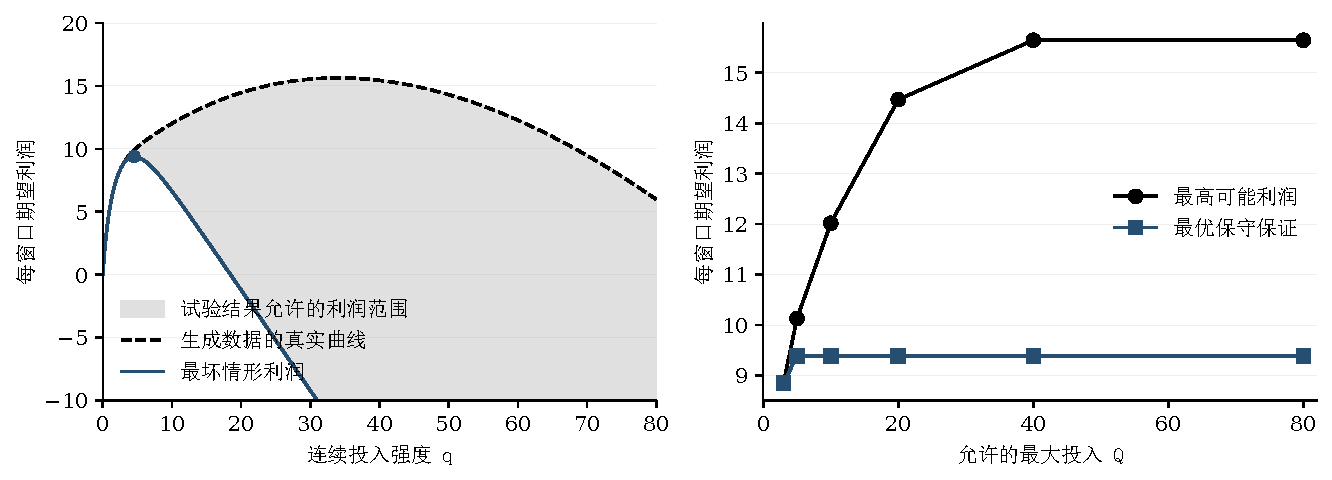
\includegraphics[width=\textwidth]{images/resource_decision.pdf}
\caption{固定的有限机会池。左图为连续投入下的净利润范围，虚线是生成数据的真实曲线，实点为保守投入；右图保持相同读数，只扩大允许部署范围。灰带是模型允许的范围，不是统计置信区间。}\label{fig:decision}
\end{figure}

为核查等距测试点并非连续投入的必要条件，还在相同机会池上测试 $0.75,1.8,3$。用奖励测度的离散线性规划求解，网格从约 500 点加密到约 8000 点，保守投入从 $4.381509$ 变为 $4.381501$，保证值从 $9.313998$ 变为 $9.313994$。这只是离散近似的收敛检查，不是任意测试设计的最优性证明，也不是对连续测度边界的认证。它表明非整数、非等距强度可以直接进入同一模型约束；等距设计的优势是有可核查的显式公式。

\subsection{从含噪计数到最终行动}
在每个窗口，两个群体分别独立命中，观测只包含捕获总数
\begin{equation}\label{eq:counts}
 Y(q)\sim\operatorname{Bin}(K-8,1-e^{-q1.4(1+\theta)/K})
       +\operatorname{Bin}(8,1-e^{-0.9q}).
\end{equation}
两项独立，$0\leq Y\leq K$；参数 $\theta\in\{0,0.05,0.1\}$ 未知。每个任务分别选择 $K\in\{100,400,1600\}$、$Q\in\{20,80\}$。算法在 $1,2,3$ 上累积观测，构造覆盖全部检查阶段的均值区间，检查模型可行性，输出连续投入，并仅在最坏情形行动损失的上界不超过 $0.5$ 时停止。附录\ref{app:computation}给出区间和停止公式。它没有使用真实的 $\theta$ 来决定何时停止。

每组独立运行 400 条路径，共 18 组、7200 条。一次成功同时要求所有已使用区间覆盖均值、程序有限停止、所选投入的保守利润距离最优保守值不超过 $0.5$。累计计数通过二项分布的可加性生成，与逐窗采样具有相同分布；没有把这些记录说成真实交易回放。

\begin{table}[H]\centering
\caption{本机重跑的完整行动程序：每行合并三个 $\theta$ 值}\label{tab:simulation}
\begin{tabular}{rrrrr}\toprule
$K$ & $Q$ & 路径数 & 记录中位数 & 最大实际行动损失\\\midrule
100 &20&1200&393216&0.003263\\
100 &80&1200&393216&0.002658\\
400 &20&1200&393216&0.003209\\
400 &80&1200&393216&0.002960\\
1600&20&1200&393216&0.002884\\
1600&80&1200&393216&0.003190\\\bottomrule
\end{tabular}
\end{table}

7200 条路径全部满足联合标准。对未合并的 18 组同时作单侧 95\% Clopper--Pearson 校正，每组成功率下界约为 $0.9854$。表\ref{tab:simulation}的最大损失是模拟中观察到的值，不是程序预先知道的保证。所有中位数相同，也部分来自样本量按倍增阶段检查，不能仅凭这些中位数断言成本严格不变。记录数仍大，且实际损失远小于停止阈值，说明充分程序保守；当前案例验证了可实现性，未证明测量成本在实际项目中合算。

除上述路径外，本机重跑了收入范围、离散矩线性规划、插值不等式和均值区间的原有检查，并为新图重新计算数据。数值规划检验实现，不能代替附录的连续测度证明。复现材料保留源程序哈希、运行日志、软件版本和新输出。有限机会池程序另在第二个独立进程重复执行，结果文件哈希一致；其逐路径输出与历史归档不完全相同，原因尚未定位，因此本文只报告本次输出，不声称历史轨迹逐条复现。

\section{用途与限制}
本模型适用于一次性奖励、稳定机会组成及可解释的有效尝试强度。合格事件的固定佣金、去重覆盖的预定价值，或固定路由下只改变搜索吞吐的任务，都可能提供这样的结构；是否成立必须由结算规则和保留强度的外样本试验检验。普通触达并不自动等于货币利润，普通交易收益也不自动满足一次奖励假设。本文没有真实平台数据，因而不把这些候选场景称为已验证应用。

实际使用时，应先固定窗口、对象、结算规则和资源计量，记录可信的总奖励上限，再交错分配若干连续强度。用未参与拟合的强度检查预测收入范围是否覆盖观测，并检查不同时间段的稳定性。若增加投入会改变机会组成，或额外群体日志、重复奖励本来就可以获得，应改写模型和信息集合。根据任务所需精度选择测量，而不是先要求恢复整条收入曲线。

本文的结论限于指定观测制度下的期望利润与稳健投入，不涉及破产概率、测量融资、任意市场漂移或竞争均衡。三个点的选择没有被证明为最优，一般连续试验设计仍待研究。两个精度要求在本文中通过同一组可行模型和收入范围相联系，更一般的统一决策理论不在本文的已完成结果之内。

\section*{代码、数据与复现}
本论文的完整源文件和附录随文提供。所有图表使用 2026 年 10 月 31 日的本机重跑结果。随文的
\href{README.md}{复现入口}提供完整运行说明、源程序和本机执行记录。
本地链接需与附件保持目录结构。当前没有公开仓库或 DOI；数据全部为合成，没有真实账户或市场连接。

\begingroup\small
\begin{thebibliography}{9}
\setlength{\itemsep}{2pt}
\bibitem{dette} Dette, H. and Studden, W. J. (1997).
\emph{The Theory of Canonical Moments with Applications in Statistics, Probability, and Analysis}. Wiley.
\bibitem{sion} Sion, M. (1958). On general minimax theorems.
\emph{Pacific Journal of Mathematics}, 8(1), 171--176.\par
\href{https://doi.org/10.2140/pjm.1958.8.171}{doi:10.2140/pjm.1958.8.171}.
\bibitem{bgk} Bertsimas, D., Gupta, V., and Kallus, N. (2018).
Data-driven robust optimization. \emph{Mathematical Programming}, 167, 235--292.\par
\href{https://doi.org/10.1007/s10107-017-1125-8}{doi:10.1007/s10107-017-1125-8}.
\bibitem{spo} Elmachtoub, A. N. and Grigas, P. (2022).
Smart ``Predict, then Optimize''. \emph{Management Science}, 68(1), 9--26.\par
\href{https://doi.org/10.1287/mnsc.2020.3922}{doi:10.1287/mnsc.2020.3922}.
\bibitem{gnedin} Gnedin, A., Hansen, B., and Pitman, J. (2007).
Notes on the occupancy problem with infinitely many boxes: general asymptotics and power laws.
\emph{Probability Surveys}, 4, 146--171.\par
\href{https://doi.org/10.1214/07-PS092}{doi:10.1214/07-PS092}.
\end{thebibliography}
\endgroup
